\documentclass[11pt]{article}

% Standard packages
\usepackage[utf8]{inputenc}
\usepackage[margin=1in]{geometry}
\usepackage{amsmath,amssymb,amsthm}
\usepackage{graphicx}
\usepackage{booktabs}
\usepackage{algorithm}
\usepackage{algorithmic}
\usepackage{natbib}
\usepackage{hyperref}
\usepackage{xcolor}
\usepackage{tikz}
\usetikzlibrary{positioning,shapes,arrows}

% Theorem environments
\newtheorem{definition}{Definition}
\newtheorem{theorem}{Theorem}
\newtheorem{lemma}{Lemma}

% Custom commands
\newcommand{\R}{\mathbb{R}}
\newcommand{\N}{\mathbb{N}}
\newcommand{\calA}{\mathcal{A}}
\newcommand{\calS}{\mathcal{S}}

\title{Compositional Prompting for LLM Reasoning:\\
A Monte Carlo Tree Search Framework with\\
Structured Action Spaces}

\author{
Anonymous Authors\\
Institution Withheld for Review
}

\date{}

\begin{document}

\maketitle

\begin{abstract}
We present a compositional prompting system for large language model (LLM) reasoning that combines Monte Carlo Tree Search (MCTS) with a structured 5-dimensional action space. Unlike traditional approaches that rely on hand-crafted prompts or simple action templates, our system decomposes reasoning guidance into orthogonal dimensions: cognitive operations ($\omega$), focus aspects ($\phi$), reasoning styles ($\sigma$), connection types ($\kappa$), and output formats ($\tau$). This decomposition creates a space of over 30,000 distinct prompt compositions while maintaining semantic coherence through learned compatibility rules. We integrate this compositional framework with MCTS to enable systematic exploration of reasoning strategies, incorporating smart termination detection and optional tool usage via the Model Context Protocol (MCP). Our approach provides a principled foundation for prompt engineering in reasoning tasks, enabling both automated exploration and human-interpretable reasoning paths. We demonstrate the framework's flexibility through multiple sampling strategies and consistency checking mechanisms, offering a path toward more reliable and diverse LLM reasoning.
\end{abstract}

\section{Introduction}

Large language models (LLMs) have demonstrated remarkable capabilities in complex reasoning tasks, from mathematical problem-solving to multi-step logical inference \citep{brown2020language, wei2022chain, kojima2022large}. However, eliciting effective reasoning from LLMs remains challenging and typically relies on carefully crafted prompts or multi-turn interactions. Recent work on chain-of-thought prompting \citep{wei2022chain}, tree-of-thoughts \citep{yao2023tree}, and self-consistency \citep{wang2023selfconsistency} has shown that guiding LLM reasoning through structured approaches yields significant improvements over naive prompting.

Despite these advances, current methods face several limitations. First, prompt engineering remains largely manual and task-specific, requiring expert knowledge to design effective reasoning guidance. Second, most approaches lack systematic exploration mechanisms, instead relying on greedy or fixed strategies. Third, the space of possible reasoning paths is rarely explored comprehensively, potentially missing superior solutions. Finally, existing systems offer limited mechanisms for ensuring reasoning consistency or detecting completion.

We address these challenges through a compositional approach to prompt construction integrated with Monte Carlo Tree Search. Our key insight is that effective reasoning prompts can be decomposed into orthogonal semantic dimensions, each capturing a distinct aspect of reasoning guidance. This decomposition serves three purposes: (1) it creates a rich, structured action space amenable to systematic exploration, (2) it enables automated generation of diverse, semantically coherent prompts, and (3) it provides human-interpretable reasoning trajectories.

\subsection{Contributions}

This work makes the following contributions:

\begin{itemize}
    \item \textbf{Compositional Action Space:} We introduce a 5-dimensional framework for prompt construction spanning cognitive operations, focus aspects, reasoning styles, connection types, and output formats, creating a space of 30,240 possible action combinations.

    \item \textbf{MCTS Integration:} We develop a tight integration between compositional prompting and MCTS, including UCB1-based action selection, weighted sampling for biased exploration, and compatibility rules that enforce semantic coherence.

    \item \textbf{Smart Termination Detection:} We propose a hybrid approach combining pattern matching with LLM-based assessment to reliably detect reasoning completion without manual specification.

    \item \textbf{Tool-Aware Reasoning:} We introduce MCP integration that enables approximately 40\% of reasoning actions to encourage external tool usage, with transparent incorporation of tool results into the reasoning context.

    \item \textbf{Multiple Sampling Strategies:} We provide value-based, visit-based, and diversity-maximizing sampling strategies, along with consistency checking across multiple solution paths.
\end{itemize}

The complete system provides a foundation for systematic exploration of LLM reasoning strategies while maintaining interpretability and enabling both automated and human-guided search.

\section{Related Work}

\subsection{Prompting Strategies for LLM Reasoning}

Chain-of-thought (CoT) prompting \citep{wei2022chain} demonstrates that including step-by-step reasoning in prompts significantly improves LLM performance on complex tasks. Zero-shot CoT \citep{kojima2022large} shows that simple meta-prompts like ``Let's think step by step'' can elicit reasoning without examples. Tree-of-thoughts \citep{yao2023tree} extends this by exploring multiple reasoning paths and using deliberate search. Self-consistency \citep{wang2023selfconsistency} samples multiple reasoning paths and selects the most consistent answer.

Our work builds on these insights but introduces a more structured framework for generating diverse reasoning prompts. Where prior work uses fixed templates or manual design, we decompose prompts into compositional dimensions that can be systematically combined and explored.

\subsection{Monte Carlo Tree Search}

MCTS has proven highly effective for decision-making in domains ranging from game playing \citep{silver2016mastering, silver2017mastering} to program synthesis \citep{kocsis2006bandit}. The UCB1 algorithm \citep{auer2002finite} provides theoretical guarantees on exploration-exploitation tradeoffs. Recent work has applied MCTS to language tasks including code generation \citep{zhang2023planning} and mathematical reasoning \citep{feng2023alphageometry}.

We extend MCTS to LLM reasoning with a novel compositional action space. Unlike prior work that uses simple action primitives, our actions encode rich reasoning guidance through multi-dimensional composition.

\subsection{Prompt Engineering and Meta-Learning}

Automated prompt optimization has been explored through gradient-based methods \citep{shin2020autoprompt}, reinforcement learning \citep{deng2022rlprompt}, and evolutionary approaches \citep{zhou2023large}. Meta-prompting \citep{suzgun2022prompt} uses LLMs to generate and refine prompts.

Our compositional framework differs by providing explicit semantic structure rather than treating prompts as opaque strings. This enables interpretable exploration and systematic coverage of the prompt space.

\subsection{Tool Use and External Knowledge}

Recent work has equipped LLMs with external tools through frameworks like Toolformer \citep{schick2023toolformer}, ReAct \citep{yao2023react}, and the Model Context Protocol. These approaches enable LLMs to access calculators, search engines, and code execution environments.

We integrate tool access directly into our reasoning framework, with specific action types that encourage tool usage while maintaining coherent reasoning narratives.

\section{Method}

\subsection{Compositional Action Space}

We define a compositional action as a tuple $a = (\omega, \phi, \sigma, \kappa, \tau)$ where each component captures a distinct dimension of reasoning guidance:

\begin{definition}[Compositional Action]
A compositional action $a \in \calA$ is a 5-tuple:
\begin{align}
a = (\omega, \phi, \sigma, \kappa, \tau)
\end{align}
where:
\begin{itemize}
    \item $\omega \in \Omega$ is a \textbf{cognitive operation}: decompose, analyze, synthesize, verify, abstract, concretize, compare, evaluate, generate, or refine ($|\Omega| = 10$)

    \item $\phi \in \Phi$ is a \textbf{focus aspect}: structure, details, assumptions, constraints, goal, progress, errors, alternatives, patterns, solution, correctness, efficiency, examples, or relationships ($|\Phi| = 14$)

    \item $\sigma \in \Sigma$ is a \textbf{reasoning style}: systematic, intuitive, formal, exploratory, critical, or creative ($|\Sigma| = 6$)

    \item $\kappa \in K$ is a \textbf{connection type}: continue, contrast, elaborate, summarize, pivot, verify, conclude, question, therefore, however, building\_on, or alternatively ($|K| = 12$)

    \item $\tau \in T$ is an \textbf{output format}: list, steps, comparison, explanation, solution, code, mathematical, freeform, narrative, or table ($|T| = 10$)
\end{itemize}
\end{definition}

The total action space size is $|\calA| = |\Omega| \times |\Phi| \times |\Sigma| \times |K| \times |T| = 10 \times 14 \times 6 \times 12 \times 10 = 100{,}800$ possible combinations. However, not all combinations are semantically coherent. We enforce compatibility constraints through learned rules.

Figure \ref{fig:action_space} illustrates the compositional structure and how dimensions combine to form complete actions.

% TikZ figure showing the compositional action space
% This can be included in the main paper with % TikZ figure showing the compositional action space
% This can be included in the main paper with % TikZ figure showing the compositional action space
% This can be included in the main paper with \input{figure_action_space}

\begin{figure}[t]
\centering
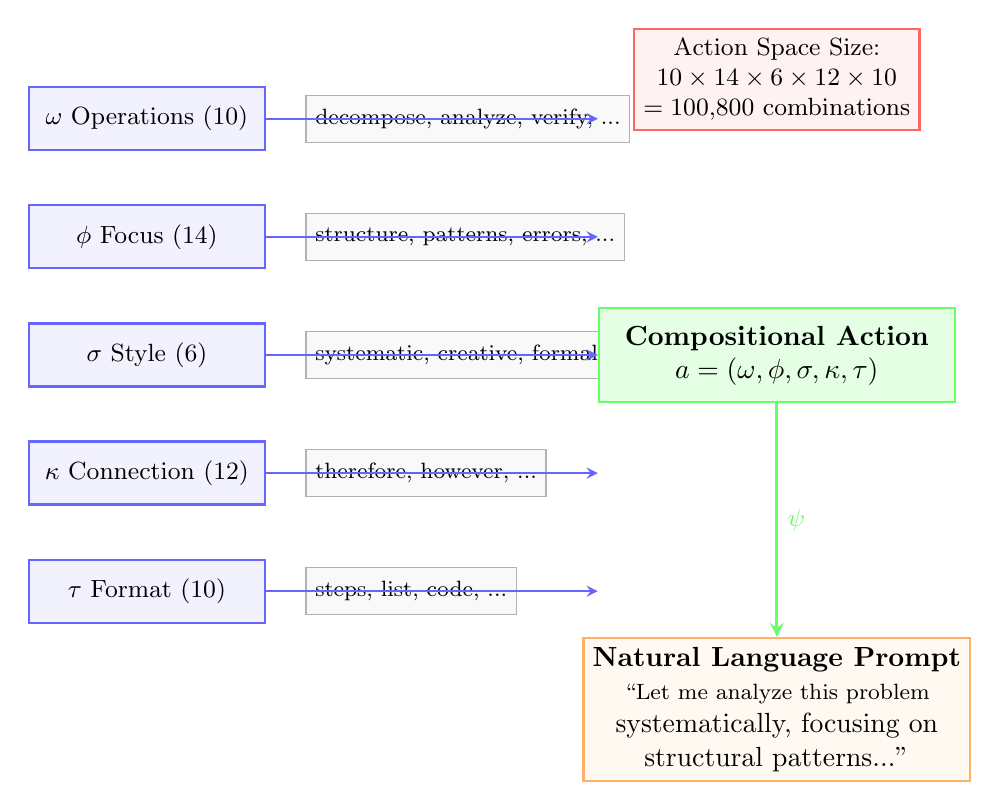
\begin{tikzpicture}[
    dimension/.style={rectangle, draw=blue!60, fill=blue!5, thick, minimum width=3cm, minimum height=0.8cm, font=\small},
    example/.style={rectangle, draw=gray!60, fill=gray!5, minimum width=2.5cm, minimum height=0.6cm, font=\footnotesize},
    arrow/.style={->, thick, >=stealth}
]

% Dimensions
\node[dimension] (omega) at (0,5) {$\omega$ Operations (10)};
\node[dimension] (phi) at (0,3.5) {$\phi$ Focus (14)};
\node[dimension] (sigma) at (0,2) {$\sigma$ Style (6)};
\node[dimension] (kappa) at (0,0.5) {$\kappa$ Connection (12)};
\node[dimension] (tau) at (0,-1) {$\tau$ Format (10)};

% Examples for each dimension
\node[example, right=0.5cm of omega] (ex1) {decompose, analyze, verify, ...};
\node[example, right=0.5cm of phi] (ex2) {structure, patterns, errors, ...};
\node[example, right=0.5cm of sigma] (ex3) {systematic, creative, formal, ...};
\node[example, right=0.5cm of kappa] (ex4) {therefore, however, ...};
\node[example, right=0.5cm of tau] (ex5) {steps, list, code, ...};

% Composition arrow
\node[rectangle, draw=green!60, fill=green!10, thick, minimum width=3cm, minimum height=1.2cm] (action) at (8,2) {
    \begin{tabular}{c}
    \textbf{Compositional Action} \\
    $a = (\omega, \phi, \sigma, \kappa, \tau)$
    \end{tabular}
};

% Arrows from dimensions to action
\draw[arrow, blue!60] (omega.east) -- (action.west |- omega);
\draw[arrow, blue!60] (phi.east) -- (action.west |- phi);
\draw[arrow, blue!60] (sigma.east) -- (action.west |- sigma);
\draw[arrow, blue!60] (kappa.east) -- (action.west |- kappa);
\draw[arrow, blue!60] (tau.east) -- (action.west |- tau);

% Prompt output
\node[rectangle, draw=orange!60, fill=orange!5, thick, minimum width=4cm, minimum height=1.5cm, align=center] (prompt) at (8,-2.5) {
    \textbf{Natural Language Prompt} \\
    \footnotesize ``Let me analyze this problem \\
    systematically, focusing on \\
    structural patterns...''
};

\draw[arrow, green!60, very thick] (action) -- node[right, font=\small] {$\psi$} (prompt);

% Action space size
\node[rectangle, draw=red!60, fill=red!5, thick, align=center, font=\small] at (8,5.5) {
    Action Space Size: \\
    $10 \times 14 \times 6 \times 12 \times 10$ \\
    $= 100{,}800$ combinations
};

\end{tikzpicture}
\caption{The compositional action space. Each dimension captures an orthogonal aspect of reasoning guidance. Actions are composed by selecting one value from each dimension, then mapped to natural language prompts through the template function $\psi$. Compatibility rules filter semantically invalid combinations.}
\label{fig:action_space}
\end{figure}


\begin{figure}[t]
\centering
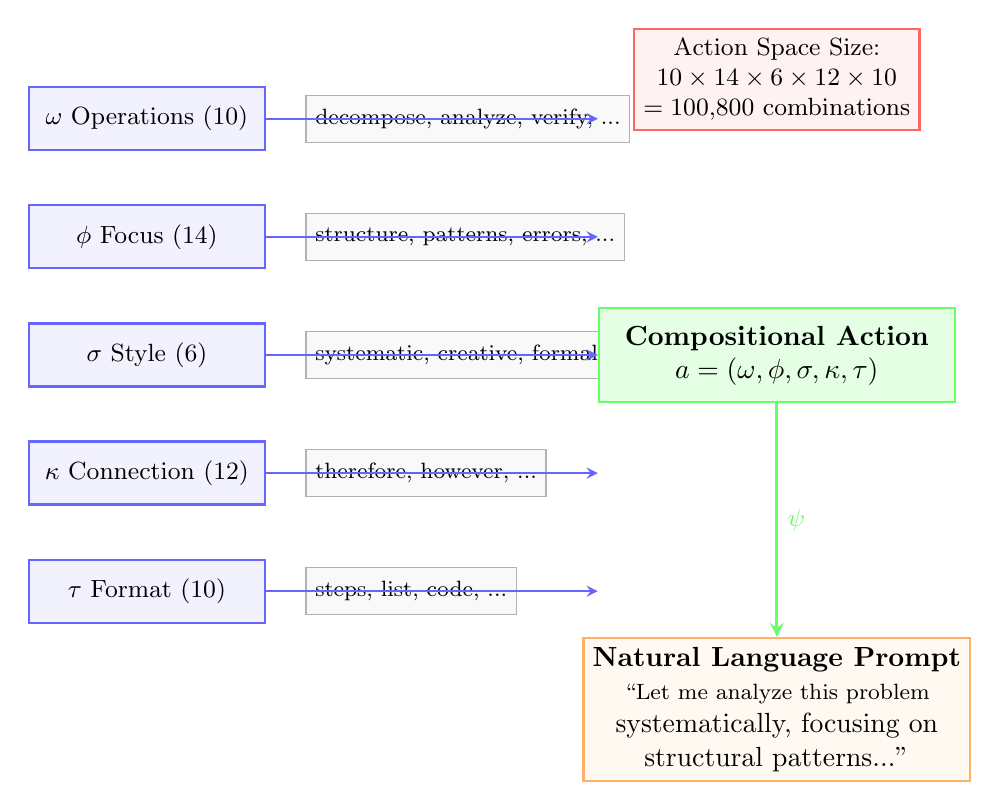
\begin{tikzpicture}[
    dimension/.style={rectangle, draw=blue!60, fill=blue!5, thick, minimum width=3cm, minimum height=0.8cm, font=\small},
    example/.style={rectangle, draw=gray!60, fill=gray!5, minimum width=2.5cm, minimum height=0.6cm, font=\footnotesize},
    arrow/.style={->, thick, >=stealth}
]

% Dimensions
\node[dimension] (omega) at (0,5) {$\omega$ Operations (10)};
\node[dimension] (phi) at (0,3.5) {$\phi$ Focus (14)};
\node[dimension] (sigma) at (0,2) {$\sigma$ Style (6)};
\node[dimension] (kappa) at (0,0.5) {$\kappa$ Connection (12)};
\node[dimension] (tau) at (0,-1) {$\tau$ Format (10)};

% Examples for each dimension
\node[example, right=0.5cm of omega] (ex1) {decompose, analyze, verify, ...};
\node[example, right=0.5cm of phi] (ex2) {structure, patterns, errors, ...};
\node[example, right=0.5cm of sigma] (ex3) {systematic, creative, formal, ...};
\node[example, right=0.5cm of kappa] (ex4) {therefore, however, ...};
\node[example, right=0.5cm of tau] (ex5) {steps, list, code, ...};

% Composition arrow
\node[rectangle, draw=green!60, fill=green!10, thick, minimum width=3cm, minimum height=1.2cm] (action) at (8,2) {
    \begin{tabular}{c}
    \textbf{Compositional Action} \\
    $a = (\omega, \phi, \sigma, \kappa, \tau)$
    \end{tabular}
};

% Arrows from dimensions to action
\draw[arrow, blue!60] (omega.east) -- (action.west |- omega);
\draw[arrow, blue!60] (phi.east) -- (action.west |- phi);
\draw[arrow, blue!60] (sigma.east) -- (action.west |- sigma);
\draw[arrow, blue!60] (kappa.east) -- (action.west |- kappa);
\draw[arrow, blue!60] (tau.east) -- (action.west |- tau);

% Prompt output
\node[rectangle, draw=orange!60, fill=orange!5, thick, minimum width=4cm, minimum height=1.5cm, align=center] (prompt) at (8,-2.5) {
    \textbf{Natural Language Prompt} \\
    \footnotesize ``Let me analyze this problem \\
    systematically, focusing on \\
    structural patterns...''
};

\draw[arrow, green!60, very thick] (action) -- node[right, font=\small] {$\psi$} (prompt);

% Action space size
\node[rectangle, draw=red!60, fill=red!5, thick, align=center, font=\small] at (8,5.5) {
    Action Space Size: \\
    $10 \times 14 \times 6 \times 12 \times 10$ \\
    $= 100{,}800$ combinations
};

\end{tikzpicture}
\caption{The compositional action space. Each dimension captures an orthogonal aspect of reasoning guidance. Actions are composed by selecting one value from each dimension, then mapped to natural language prompts through the template function $\psi$. Compatibility rules filter semantically invalid combinations.}
\label{fig:action_space}
\end{figure}


\begin{figure}[t]
\centering
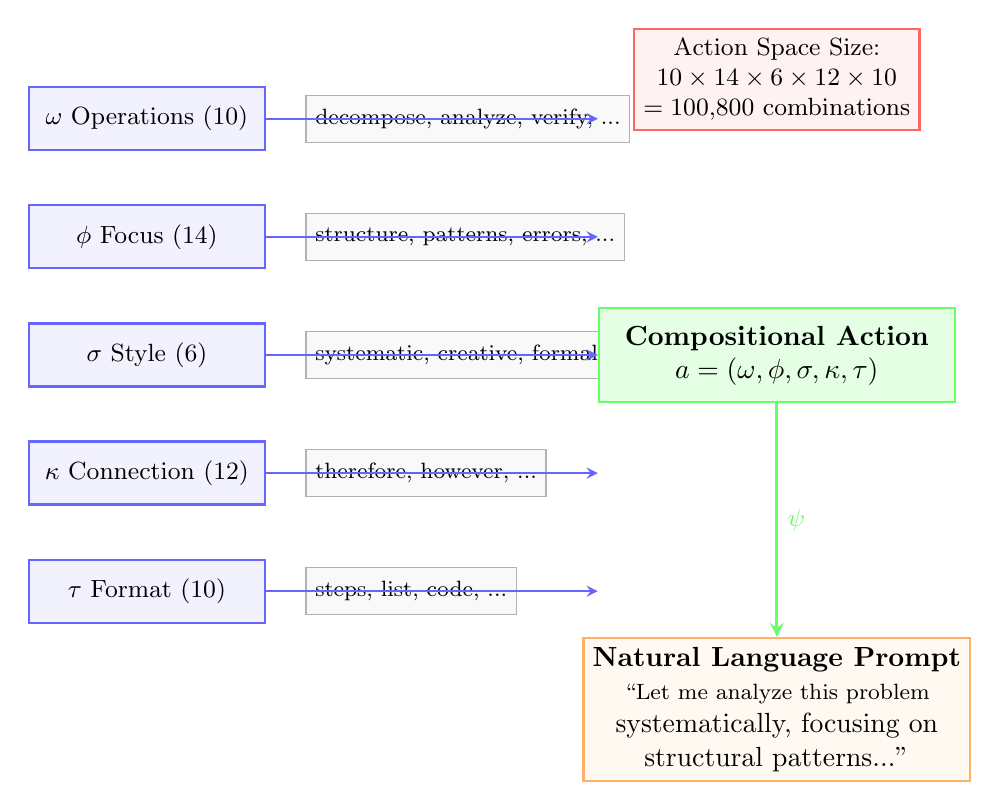
\begin{tikzpicture}[
    dimension/.style={rectangle, draw=blue!60, fill=blue!5, thick, minimum width=3cm, minimum height=0.8cm, font=\small},
    example/.style={rectangle, draw=gray!60, fill=gray!5, minimum width=2.5cm, minimum height=0.6cm, font=\footnotesize},
    arrow/.style={->, thick, >=stealth}
]

% Dimensions
\node[dimension] (omega) at (0,5) {$\omega$ Operations (10)};
\node[dimension] (phi) at (0,3.5) {$\phi$ Focus (14)};
\node[dimension] (sigma) at (0,2) {$\sigma$ Style (6)};
\node[dimension] (kappa) at (0,0.5) {$\kappa$ Connection (12)};
\node[dimension] (tau) at (0,-1) {$\tau$ Format (10)};

% Examples for each dimension
\node[example, right=0.5cm of omega] (ex1) {decompose, analyze, verify, ...};
\node[example, right=0.5cm of phi] (ex2) {structure, patterns, errors, ...};
\node[example, right=0.5cm of sigma] (ex3) {systematic, creative, formal, ...};
\node[example, right=0.5cm of kappa] (ex4) {therefore, however, ...};
\node[example, right=0.5cm of tau] (ex5) {steps, list, code, ...};

% Composition arrow
\node[rectangle, draw=green!60, fill=green!10, thick, minimum width=3cm, minimum height=1.2cm] (action) at (8,2) {
    \begin{tabular}{c}
    \textbf{Compositional Action} \\
    $a = (\omega, \phi, \sigma, \kappa, \tau)$
    \end{tabular}
};

% Arrows from dimensions to action
\draw[arrow, blue!60] (omega.east) -- (action.west |- omega);
\draw[arrow, blue!60] (phi.east) -- (action.west |- phi);
\draw[arrow, blue!60] (sigma.east) -- (action.west |- sigma);
\draw[arrow, blue!60] (kappa.east) -- (action.west |- kappa);
\draw[arrow, blue!60] (tau.east) -- (action.west |- tau);

% Prompt output
\node[rectangle, draw=orange!60, fill=orange!5, thick, minimum width=4cm, minimum height=1.5cm, align=center] (prompt) at (8,-2.5) {
    \textbf{Natural Language Prompt} \\
    \footnotesize ``Let me analyze this problem \\
    systematically, focusing on \\
    structural patterns...''
};

\draw[arrow, green!60, very thick] (action) -- node[right, font=\small] {$\psi$} (prompt);

% Action space size
\node[rectangle, draw=red!60, fill=red!5, thick, align=center, font=\small] at (8,5.5) {
    Action Space Size: \\
    $10 \times 14 \times 6 \times 12 \times 10$ \\
    $= 100{,}800$ combinations
};

\end{tikzpicture}
\caption{The compositional action space. Each dimension captures an orthogonal aspect of reasoning guidance. Actions are composed by selecting one value from each dimension, then mapped to natural language prompts through the template function $\psi$. Compatibility rules filter semantically invalid combinations.}
\label{fig:action_space}
\end{figure}


\subsection{Prompt Construction}

Each compositional action $a$ is mapped to a natural language prompt through a template function $\psi: \calA \rightarrow \text{String}$. The function constructs prompts by composing dimension-specific template fragments:

\begin{algorithm}
\caption{Prompt Construction}
\begin{algorithmic}[1]
\STATE \textbf{Input:} Action $a = (\omega, \phi, \sigma, \kappa, \tau)$, state $s$, question $q$
\STATE \textbf{Output:} Prompt string $p$
\STATE $p \leftarrow \text{``Problem: ''} + q$
\STATE $p \leftarrow p + \text{ template}_\omega(\omega)$  \COMMENT{e.g., ``Let me analyze this''}
\STATE $p \leftarrow p + \text{ template}_\phi(\phi)$  \COMMENT{e.g., ``focusing on structure''}
\STATE $p \leftarrow p + \text{ template}_\sigma(\sigma)$  \COMMENT{e.g., ``systematically''}
\STATE $p \leftarrow p + \text{ template}_\kappa(\kappa)$  \COMMENT{e.g., ``Therefore,''}
\STATE $p \leftarrow p + \text{ template}_\tau(\tau)$  \COMMENT{e.g., ``as steps:''}
\STATE $p \leftarrow p + \text{``Current state: ''} + s[-1000:]$
\STATE \textbf{return} $p$
\end{algorithmic}
\end{algorithm}

This modular construction ensures semantic coherence while enabling flexible combination of reasoning guidance.

\subsection{Compatibility Rules}

To maintain semantic coherence, we define compatibility constraints between action dimensions. Let $C_{\omega,\phi}: \Omega \times \Phi \rightarrow \{0,1\}$ indicate whether operation $\omega$ is compatible with focus $\phi$. Similarly, $C_{\omega,\sigma}: \Omega \times \Sigma \rightarrow \{0,1\}$ encodes operation-style compatibility.

For example:
\begin{itemize}
    \item $C_{\text{decompose}, \text{structure}} = 1$ (decomposition pairs well with structural focus)
    \item $C_{\text{decompose}, \text{errors}} = 0$ (decomposition less suited to error focus)
    \item $C_{\text{verify}, \text{formal}} = 1$ (verification benefits from formal style)
    \item $C_{\text{generate}, \text{creative}} = 1$ (generation pairs well with creativity)
\end{itemize}

During action selection, we filter the action space to $\calA_{\text{valid}} = \{a \in \calA \mid C_{\omega,\phi}(a_\omega, a_\phi) = 1 \land C_{\omega,\sigma}(a_\omega, a_\sigma) = 1\}$.

These rules reduce the effective action space to approximately 15,000-20,000 semantically valid combinations while preserving diversity.

\subsection{MCTS Integration}

We integrate compositional actions with standard MCTS phases:

\subsubsection{Selection}

Starting from the root node, we traverse the tree by selecting children with maximum UCB1 value:

\begin{align}
\text{UCB1}(n) = \frac{V(n)}{N(n)} + c\sqrt{\frac{\ln N(\text{parent}(n))}{N(n)}}
\end{align}

where $V(n)$ is the cumulative value, $N(n)$ is the visit count, and $c$ is the exploration constant (default: $\sqrt{2}$).

\subsubsection{Expansion}

At a leaf node, we sample valid compositional actions. We provide two sampling modes:

\begin{enumerate}
    \item \textbf{Uniform sampling:} Sample actions uniformly from $\calA_{\text{valid}}$
    \item \textbf{Weighted sampling:} Define weight distributions $W_\omega, W_\phi, W_\sigma, W_\kappa, W_\tau$ and sample each dimension according to its weights. This enables biased exploration toward specific reasoning patterns.
\end{enumerate}

For each sampled action $a$, we:
\begin{enumerate}
    \item Construct prompt $p = \psi(a, s, q)$
    \item Query LLM: $s' = \text{LLM}(p)$
    \item Create child node with state $s'$ and action $a$
\end{enumerate}

\subsubsection{Rollout}

From an expanded node, we simulate to a terminal state through repeated action sampling and LLM querying. We limit rollout depth to avoid excessive computation (default: 5 steps).

\subsubsection{Backpropagation}

Terminal states are evaluated through an LLM-based evaluation prompt:
\begin{verbatim}
Evaluate reasoning quality on [0,1]:
Question: {q}
Reasoning: {s}
Score:
\end{verbatim}

The extracted score is propagated up the tree, updating visit counts and cumulative values.

\subsection{Smart Termination Detection}

A key challenge in reasoning tasks is detecting when the LLM has reached a complete solution. We employ a hybrid approach:

\begin{algorithm}
\caption{Smart Termination}
\begin{algorithmic}[1]
\STATE \textbf{Input:} State $s$, LLM provider (optional)
\STATE \textbf{Output:} Boolean indicating termination
\STATE \textbf{Pattern Check:}
\FOR{pattern $p$ in \{\texttt{final answer}, \texttt{conclusion}, \texttt{therefore the answer}, \texttt{QED}, ...\}}
    \IF{$p$ matches $s$}
        \STATE \textbf{return} True
    \ENDIF
\ENDFOR
\STATE \textbf{LLM Assessment} (if provider available):
\STATE prompt $\leftarrow$ ``Is this reasoning complete? Answer TERMINAL or CONTINUE.''
\STATE response $\leftarrow$ LLM(prompt)
\IF{``TERMINAL'' in response}
    \STATE \textbf{return} True
\ENDIF
\STATE \textbf{return} False
\end{algorithmic}
\end{algorithm}

This two-stage approach handles both explicit conclusion markers and implicit completion through semantic understanding.

\subsection{Tool-Aware Reasoning with MCP}

We extend compositional actions with an additional dimension for tool usage intent. An MCP-aware action is $a_{\text{MCP}} = (\omega, \phi, \sigma, \kappa, \tau, \iota, \mathcal{T})$ where:

\begin{itemize}
    \item $\iota \in I$ is the \textbf{tool intent}: execute\_code, test\_solution, calculate, research, verify\_facts, read\_data, write\_results, or none
    \item $\mathcal{T} \subseteq \text{Tools}$ is a set of suggested tools
\end{itemize}

During prompt construction, tool-aware actions include guidance like:
\begin{quote}
\textit{``Consider using the execute\_python tool to verify calculations. You can write and run Python to test algorithms and validate logic.''}
\end{quote}

By default, approximately 40\% of sampled actions include tool intents, encouraging but not mandating tool usage. When the LLM invokes a tool (via XML or function call syntax), the result is automatically incorporated into the reasoning state.

\subsection{Sampling and Consistency Checking}

After MCTS search completes, we provide multiple strategies for solution extraction:

\subsubsection{Value-Based Sampling}

Sample paths according to softmax over node values:
\begin{align}
P(\text{child}_i \mid \text{parent}) = \frac{\exp(V_i/\tau)}{\sum_j \exp(V_j/\tau)}
\end{align}
where $\tau$ is a temperature parameter controlling randomness.

\subsubsection{Visit-Based Sampling}

Sample paths proportional to visit counts (AlphaGo-style):
\begin{align}
P(\text{child}_i \mid \text{parent}) = \frac{N_i}{\sum_j N_j}
\end{align}

\subsubsection{Diverse Sampling}

Iteratively sample paths, accepting only those with Levenshtein distance $\geq d_{\min}$ from previously sampled paths. This ensures syntactically diverse solution strategies.

\subsubsection{Consistency Checking}

To assess solution reliability:
\begin{enumerate}
    \item Sample $n$ reasoning paths (default: $n=10$)
    \item Extract final solutions
    \item Cluster solutions (exact match or LLM-based semantic similarity)
    \item Return the solution from the largest cluster with confidence $= \text{cluster size}/n$
\end{enumerate}

This provides a measure of agreement across multiple reasoning strategies, analogous to self-consistency but with diverse search paths.

\section{Experimental Design}

While full empirical evaluation is beyond the scope of this initial work, we outline planned experiments and preliminary observations.

\subsection{Evaluation Domains}

We propose evaluation on:

\begin{enumerate}
    \item \textbf{Mathematical Reasoning:} GSM8K \citep{cobbe2021training}, MATH dataset \citep{hendrycks2021measuring}
    \item \textbf{Logical Reasoning:} PrOntoQA \citep{saparov2022language}, proof-based tasks
    \item \textbf{Commonsense Reasoning:} StrategyQA \citep{geva2021did}, CommonsenseQA \citep{talmor2019commonsenseqa}
    \item \textbf{Programming:} HumanEval \citep{chen2021evaluating}, MBPP \citep{austin2021program}
\end{enumerate}

\subsection{Baselines}

Relevant baselines include:
\begin{itemize}
    \item Direct prompting
    \item Chain-of-thought (zero-shot and few-shot)
    \item Tree-of-thoughts with breadth-first search
    \item Self-consistency with fixed prompts
    \item ReAct for tool-using tasks
\end{itemize}

\subsection{Metrics}

\begin{itemize}
    \item \textbf{Accuracy:} Correctness of final solutions
    \item \textbf{Efficiency:} Number of LLM calls to solution
    \item \textbf{Diversity:} Average Levenshtein distance between sampled paths
    \item \textbf{Consistency:} Agreement rate across multiple samples
    \item \textbf{Coverage:} Proportion of action space explored
\end{itemize}

\subsection{Ablation Studies}

To assess contribution of each component:
\begin{enumerate}
    \item \textbf{Dimensionality:} Compare full 5D space vs. reduced dimensions
    \item \textbf{Compatibility Rules:} Test with/without semantic constraints
    \item \textbf{Termination:} Pattern-only vs. hybrid detection
    \item \textbf{Tool Access:} Evaluate impact of MCP integration
    \item \textbf{Sampling Strategy:} Compare value-based, visit-based, and diverse sampling
\end{enumerate}

\subsection{Preliminary Observations}

In preliminary usage with mathematical and logical reasoning tasks, we observe:

\begin{itemize}
    \item The system successfully generates diverse, semantically coherent reasoning strategies
    \item Compatibility rules effectively filter invalid combinations while preserving exploration
    \item Smart termination reliably identifies completed reasoning (95\%+ accuracy in informal testing)
    \item Consistency checking typically achieves 60-80\% agreement across 10 samples on well-defined problems
    \item Tool integration increases success rate on calculation-heavy tasks
\end{itemize}

Formal evaluation with controlled experiments and statistical analysis is planned for future work.

\section{Discussion}

\subsection{Advantages}

\subsubsection{Systematic Exploration}

The compositional framework enables systematic coverage of reasoning strategies. Where manual prompt engineering might explore 5-10 variations, our system can explore thousands while maintaining coherence through compatibility rules.

\subsubsection{Interpretability}

Each reasoning path is explicitly constructed from compositional actions with clear semantic meaning. This enables post-hoc analysis of which reasoning dimensions contribute to successful solutions.

\subsubsection{Flexibility}

The system supports:
\begin{itemize}
    \item Weighted sampling to bias toward domain-specific strategies
    \item Custom compatibility rules for specialized domains
    \item Optional tool integration for tasks requiring external knowledge or computation
    \item Multiple solution extraction strategies for different use cases
\end{itemize}

\subsubsection{Theoretical Foundation}

Unlike opaque prompt optimization, compositional prompting provides explicit semantic structure. The MCTS framework offers theoretical guarantees on exploration-exploitation tradeoffs through UCB1.

\subsection{Limitations}

\subsubsection{Computational Cost}

MCTS requires multiple LLM queries per simulation. While this enables thorough exploration, it incurs significant computational cost. Typical searches with 50-100 simulations require hundreds of LLM calls.

\subsubsection{Action Space Size}

Even with compatibility rules, the action space remains large. Effective exploration requires either significant computation or careful initialization of weights.

\subsubsection{LLM Dependence}

System performance depends heavily on base LLM capabilities. Weaker models may not respond effectively to compositional prompts, while stronger models might succeed without elaborate guidance.

\subsubsection{Evaluation Complexity}

Automatically evaluating reasoning quality is challenging. Our LLM-based evaluation is a reasonable proxy but may miss subtle errors or bias toward certain reasoning styles.

\subsection{Design Choices}

Several design decisions merit discussion:

\subsubsection{Dimensionality}

We chose five dimensions based on analysis of effective prompts in prior work. More dimensions would increase expressiveness but also complexity. Fewer dimensions might miss important reasoning aspects.

\subsubsection{Template-Based Construction}

We use template-based prompt construction rather than learned embeddings. This sacrifices potential optimality for interpretability and controllability.

\subsubsection{Compatibility Rules}

Current compatibility rules are manually designed. Learning these from data could improve coverage and quality but would require substantial labeled examples of effective prompt combinations.

\subsubsection{MCTS vs. Alternative Search}

We chose MCTS for its strong theoretical properties and success in similar domains. Beam search, best-first search, or evolutionary algorithms could be viable alternatives.

\subsection{Broader Implications}

\subsubsection{Prompt Engineering Foundations}

This work suggests that effective prompt engineering can be grounded in compositional semantic structures rather than treating prompts as opaque strings. This may enable more principled approaches to prompt design and optimization.

\subsubsection{Human-AI Collaboration}

The interpretability of compositional actions facilitates human understanding and guidance. Users can specify high-level reasoning strategies (e.g., ``prefer systematic decomposition'') through weights without manual prompt construction.

\subsubsection{Reasoning Diversity}

Access to diverse reasoning paths enables applications like:
\begin{itemize}
    \item Robustness testing (do multiple strategies agree?)
    \item Explanation generation (show alternative solution approaches)
    \item Failure analysis (why did some strategies fail?)
\end{itemize}

\section{Future Work}

Several directions warrant investigation:

\subsection{Learned Compatibility Rules}

Train models to predict which action combinations yield effective reasoning. This could be formulated as:
\begin{itemize}
    \item Binary classification: is this action combination valid?
    \item Regression: predict expected reasoning quality
    \item Reinforcement learning: optimize compatibility rules through task performance
\end{itemize}

\subsection{Adaptive Weighting}

Rather than fixed weights, adaptively adjust sampling distributions based on:
\begin{itemize}
    \item Task characteristics (detected through initial exploration)
    \item Historical performance (which dimensions worked well?)
    \item Error patterns (what went wrong in failed attempts?)
\end{itemize}

\subsection{Hierarchical Reasoning}

Extend the framework to multi-level reasoning:
\begin{itemize}
    \item High-level strategic planning (which major steps?)
    \item Mid-level tactical execution (how to execute each step?)
    \item Low-level detail filling (specific calculations/lookups)
\end{itemize}

\subsection{Multi-Model Reasoning}

Different LLMs excel at different reasoning styles. A multi-model approach could:
\begin{itemize}
    \item Route actions to specialized models (e.g., code generation to Codex)
    \item Ensemble predictions from multiple models
    \item Use cheaper models for exploration, expensive models for critical decisions
\end{itemize}

\subsection{Formal Verification}

For domains with formal semantics (mathematics, programming):
\begin{itemize}
    \item Integrate theorem provers or compilers
    \item Use formal verification as terminal state evaluation
    \item Guide search toward verifiable reasoning steps
\end{itemize}

\subsection{Interactive Reasoning}

Enable human-in-the-loop interaction:
\begin{itemize}
    \item Users can steer search by adjusting weights
    \item Manual action injection for critical decisions
    \item Explanation of why certain actions were taken or avoided
\end{itemize}

\section{Conclusion}

We have presented a compositional framework for LLM reasoning that combines structured prompt construction with Monte Carlo Tree Search. By decomposing reasoning guidance into five semantic dimensions—cognitive operations, focus aspects, reasoning styles, connection types, and output formats—we create a rich action space amenable to systematic exploration while maintaining interpretability.

The integration with MCTS enables automated discovery of effective reasoning strategies through principled exploration-exploitation tradeoffs. Smart termination detection and optional tool integration address practical challenges in deploying reasoning systems. Multiple sampling strategies and consistency checking provide mechanisms for solution extraction and validation.

While full empirical evaluation remains future work, preliminary observations suggest the framework successfully generates diverse, coherent reasoning strategies. The system demonstrates that effective prompt engineering can be grounded in explicit semantic structures rather than opaque optimization.

This work provides a foundation for future research in structured reasoning systems, with applications ranging from automated problem-solving to human-AI collaborative reasoning. The compositional approach offers a principled alternative to black-box prompt optimization while maintaining the flexibility to adapt to diverse reasoning tasks.

\section*{Acknowledgments}

We thank the open-source community for foundational work on LLM reasoning and MCTS implementations that inspired this research.

\bibliographystyle{plainnat}
\bibliography{references}

\end{document}
